\documentclass[hidelinks,12pt]{article}
\usepackage[left=0.25cm,top=1cm,right=0.25cm,bottom=1cm]{geometry}
%\usepackage[landscape]{geometry}
\textwidth = 20cm
\hoffset = -1cm
\usepackage[utf8]{inputenc}
\usepackage[spanish,es-tabla]{babel}
\usepackage[autostyle,spanish=mexican]{csquotes}
\usepackage[tbtags]{amsmath}
\usepackage{nccmath}
\usepackage{amsthm}
\usepackage{amssymb}
\usepackage{mathrsfs}
\usepackage{graphicx}
\usepackage{subfig}
\usepackage{standalone}
\usepackage[outdir=./Imagenes/]{epstopdf}
\usepackage{siunitx}
\usepackage{physics}
\usepackage{color}
\usepackage{float}
\usepackage{hyperref}
\usepackage{multicol}
%\usepackage{milista}
\usepackage{anyfontsize}
\usepackage{anysize}
%\usepackage{enumerate}
\usepackage[shortlabels]{enumitem}
\usepackage{capt-of}
\usepackage{bm}
\usepackage{relsize}
\usepackage{placeins}
\usepackage{empheq}
\usepackage{cancel}
\usepackage{wrapfig}
\usepackage[flushleft]{threeparttable}
\usepackage{makecell}
\usepackage{fancyhdr}
\usepackage{tikz}
\usepackage{bigints}
\usepackage{scalerel}
\usepackage{pgfplots}
\usepackage{pdflscape}
\pgfplotsset{compat=1.16}
\spanishdecimal{.}
\renewcommand{\baselinestretch}{1.5} 
\renewcommand\labelenumii{\theenumi.{\arabic{enumii}})}
\newcommand{\ptilde}[1]{\ensuremath{{#1}^{\prime}}}
\newcommand{\stilde}[1]{\ensuremath{{#1}^{\prime \prime}}}
\newcommand{\ttilde}[1]{\ensuremath{{#1}^{\prime \prime \prime}}}
\newcommand{\ntilde}[2]{\ensuremath{{#1}^{(#2)}}}

\newtheorem{defi}{{\it Definición}}[section]
\newtheorem{teo}{{\it Teorema}}[section]
\newtheorem{ejemplo}{{\it Ejemplo}}[section]
\newtheorem{propiedad}{{\it Propiedad}}[section]
\newtheorem{lema}{{\it Lema}}[section]
\newtheorem{cor}{Corolario}
\newtheorem{ejer}{Ejercicio}[section]

\newlist{milista}{enumerate}{2}
\setlist[milista,1]{label=\arabic*)}
\setlist[milista,2]{label=\arabic{milistai}.\arabic*)}
\newlength{\depthofsumsign}
\setlength{\depthofsumsign}{\depthof{$\sum$}}
\newcommand{\nsum}[1][1.4]{% only for \displaystyle
    \mathop{%
        \raisebox
            {-#1\depthofsumsign+1\depthofsumsign}
            {\scalebox
                {#1}
                {$\displaystyle\sum$}%
            }
    }
}
\def\scaleint#1{\vcenter{\hbox{\scaleto[3ex]{\displaystyle\int}{#1}}}}
\def\bs{\mkern-12mu}


%\usepackage{showframe}
\usepackage{apacite}
\title{Operador momento angular \\ \large {Tema 4 - Sep. variables en coord. esféricas} \vspace{-3ex}}
\author{M. en C. Gustavo Contreras Mayén}
\date{ }
\begin{document}
\vspace{-4cm}
\maketitle
\fontsize{14}{14}\selectfont
\tableofcontents
\newpage
\section{Introducción.}
En mecánica clásica, el momento angular $\vb{L}$, se define como:
\begin{align}
\vb{L} = \va{r} \cp \va{p}
\label{eq:ecuacion_05_05}
\end{align}
donde
\begin{align*}
\va{r} &= x \, \vu{i} + j \, \vu{j} + z \, \vu{k} \\[0.5em]
\va{p} &= m \left( v_{x} \, \vu{i} + v_{j} \, \vu{j} + v_{z} \, \vu{k} \right) = p_{x} \, \vu{i} + p_{y} \, \vu{j} + p_{z} \, \vu{k}
\end{align*}
Por lo que:
\begin{align}
\begin{aligned}
\va{L} = \mdet{
\vu{i} & \vu{j} & \vu{k} \\
x & y & z \\
p_{x} & p_{y} & p_{z}
} &= ( y \, p_{z} - z \, p_{y}) \, \vu{i} + ( z \, p_{x} - x \, p_{z}) \, \vu{j} + ( x \, p_{y} - y \, p_{x}) \, \vu{k} = \\[0.5em]
&= L_{x} \, \vu{i} + L_{y} \, \vu{j} + L_{z} \, \vu{k}
\end{aligned}
\label{eq:ecuacion_05_06}
\end{align}
El cuadrado del módulo del vector momento angular será
\begin{align}
L^{2} = L_{x}^{2} L_{y}^{2} + L_{z}^{2}
\label{eq:ecuacion_05_07}
\end{align}
En mecánica cuántica el operador momento angular se define también según la ecuación (\ref{eq:ecuacion_05_06}), con la salvedad de que ahora, los momentos lineales $p_{x}$, $p_{y}$ y $p{z}$ toman sus expresiones cuánticas  $p_{i} = -i \hbar \pdv*{x_{i}}$. Por lo tanto: 
\begin{align}
L_{x} = y \, p_{z} - z \, p_{y}, \hspace{1cm} L_{y} = z \, p_{x} - x \, p_{z} \hspace{1cm} L_{z} = x \, p_{y} - y \, p_{x} 
\end{align}
Las componentes del vector momento angular no conmutan entre sí. Como ejemplo veamos el valor de $[L_{x}, L_{y}]$:
\begin{align}
\begin{aligned}[b]
[L_{x} , L_{y}] &= (y \, p_{z} - z \, p_{y}), (z \, p_{x} - x \, p_{z})] = \\[0.5em]
&= [y \, p_{z} , z \, p_{x}] - [y \, p_{z}, x \, p_{z}] -  [z \, p_{y}, z \, p_{x}] + [z \, p_{y}, x \, p_{z}]
\end{aligned}
\label{eq:ecuacion_05_09}
\end{align}
Ahora, es necesario analizar el valor de cada uno de estos cuatro conmutadores que aparecen en la expresión anterior. Para ello, hay que tener en cuenta que $p_{x} \, y = 0$ etc, es decir las coordenadas son linealmente independientes. Así, por ejemplo una operación como
\begin{align*}
y \, p_{z} \, x \, p_{z} = y \, x \, p_{z}^{2}
\end{align*}
ya que $x$ es independiente de $z$. Además $[p_{x}, x] = - i \hbar$, y lo mismo con las coordenadas $y$ y $z$. Luego:
\begin{align}
\begin{aligned}
[y \, p_{z}, z \, p_{x}] &= y \, p_{z} \, z \, p_{x} - z \, p_{x} \, y \, p_{z} = y \, p_{z} \, z \, p_{x} - y \, z \, p_{z} \, p_{x} = \\[0.5em]
&= y \, [p_{z}, z] \, p_{x} = -i \, \hbar \, y \, p_{x} \\[0.5em]
[y \, p_{z}, x \, p_{z}] &= y \, p_{z} \, x \, p_{z} - x \, p_{z} \, y \, p_{z} = x \, y \, p_{z}^{2} - x \, y \, p_{z}^{2} = 0 \\[0.5em]
[z \, p_{y}, z \, p_{x}] &= z \, p_{y} \, z \, p_{x} - z \, p_{x} \, z \, p_{y} = z^{2} \, p_{y} \, p_{x} - z^{2} \, p_{y} \, p_{x} = 0 \\[0.5em]
[z \, p_{y}, x \, p_{z}] &= z \, p_{y} \, x \, p_{z} - x \, p_{z} \, z \, p_{y} = x \, p_{y} \, z \, p_{z} - x \, p_{y} \, p_{z} \, z = \\[0.5em]
&= - x \, p_{y} \, [p_{z}, z] = -i \, \hbar \, x \, p_{y}
\end{aligned}
\label{eq:ecuacion_05_10}
\end{align}
por lo tanto:
\begin{align}
[L_{x}, L_{y}] = i \, \hbar (- y \, p_{x} + x \, p_{y}) = - i \, \hbar \, L_{z}
\label{eq:ecuacion_05_11}
\end{align}
de la misma forma, puede demostrarse que:
\begin{align}
[L_{x}, L_{y}] = i \, \hbar \, L_{z} \hspace{1cm} [L_{y}, L_{z}] = i \, \hbar \, L_{x} \hspace{1cm} [L_{z}, L_{x}] = i \, \hbar \, L_{y}
\label{eq:ecuacion_05_12}
\end{align}
Al no conmutar los operadores, las observables correspondientes no pueden ser determinadas simultáneamente. Físicamente esto significa que, al ser imposible determinar con precisión dos de las componentes de un vector, también será imposible determinar con precisión la orientación de dicho vector. Por el contrario, el operador $\vb{L}^{2}$, si conmuta con cualquiera de sus componentes.
\par
Calculemos $[\vb{L}^{2}, L_{x}]$:
\begin{align}
[\vb{L}^{2}, L_{x}] = [{L}_{x}^{2}, L_{x}] + [{L}_{y}^{2}, L_{x}] + [{L}_{z}^{2}, L_{x}]
\label{eq:ecuacion_05_13}
\end{align} 
Evidentemente se tiene que:
\begin{align*}
[\vb{L}_{x}^{2}, L_{x}] = 0
\end{align*}
Mientras que los otros conmutadores:
\begin{subequations}
\begin{align}
\begin{aligned}[b]
[\vb{L}_{y}^{2}, L_{x}] &= L_{y} \, L_{y} \, L_{x} - L_{x} \, L_{y} \, L_{y} + L_{y} \, L_{x} \, L_{y} - L_{y} \, L_{x} \, L_{y} =  \\[0.5em]
&= L_{y} \, [L_{y} , L_{x}] + [L_{y} , L_{x}] \, L_{x} = \\[0.5em]
&= - i \, \hbar (L_{y} \, L_{z} + L_{z} \, L_{y})
\end{aligned}
\label{eq:ecuacion_0514a}
\end{align}
\begin{align}
\begin{aligned}[b]
[\vb{L}_{z}^{2}, L_{x}] &= L_{z} \, L_{z} \, L_{x} - L_{x} \, L_{z} \, L_{z} + L_{z} \, L_{x} \, L_{z} - L_{z} \, L_{x} \, L_{z} =  \\[0.5em]
&= L_{z} \, [L_{z} , L_{x}] + [L_{z} , L_{x}] \, L_{z} = \\[0.5em]
&= i \, \hbar (L_{z} \, L_{y} + L_{y} \, L_{z})
\end{aligned}
\label{eq:ecuacion_0514b}
\end{align}
\end{subequations}
Por lo que $[\vb{L}^{2}, L_{x}] = 0$, de la misma forma puede demostrarse que:
\begin{align}
[\vb{L}^{2}, L_{x}] = [\vb{L}^{2}, L_{y}] = [\vb{L}^{2}, L_{z}] = 0
\label{eq:ecuacion_05_15}
\end{align}
Es decir, el módulo del vector $\vb{L}$ y cualquiera de sus proyecciones pueden determinarse simultáneamente. Gran importancia tienen las expresiones de estos operadores en coordenadas esféricas polares:
\begin{align}
L_{x} &= i \, \hbar \left( \sin \phi \, \pdv{\theta} + \cot \theta \, \cos \phi \, \pdv{\phi} \right) \label{eq:ecuacion_05_16} \\[0.5em]
L_{y} &= - i \, \hbar \left( \cos \phi \, \pdv{\theta} - \cot \theta \, \sin \phi \, \pdv{\phi} \right) \label{eq:ecuacion_05_17} \\[0.5em]
L_{z} &= - i \, \hbar \, \pdv{\phi} \label{eq:ecuacion_05_18} \\[0.5em]
\vb{L}^{2} &= - \hbar^{2} \left( \dfrac{1}{\sen \theta} \, \pdv{\theta} \left( \sin \theta \, \pdv{\theta} \right) + \dfrac{1}{\sin^{2} \theta} \, \pdv[2]{\phi} \right) \label{eq:ecuacion_05_19}
\end{align}
%Ref. Griffiths (2005) - 4.3.1
Entonces $\vb{L}^{2}$ es compatible con cada componente de $\vb{L}$, y podemos esperar encontrar estados propios simultáneos de $\vb{L}^{2}$ y (digamos) $L_{z}$:
\begin{align}
\vb{L}^{2} \, f = \lambda \, f \hspace{1cm} \mbox{y} \hspace{1cm} L_{z} \, f = \mu \, f
\label{eq:ecuacion_04_104}
\end{align}
\section{Operadores de escalera.}
Usando una técnica de \emph{operador de escalera}, dejando que:
\begin{align}
L_{\pm} \equiv L_{x} \pm i \, L_{y}
\label{eq:ecuacion_04_105}
\end{align}
El conmutador con $L_{z}$ es:
\begin{align*}
[L_{z}, L_{\pm}] &= [L_{z}, L_{x}] \pm i \, [L_{z}, L_{y}] = \\[0.5em]
&= i \, \hbar \, L_{y} \pm i \, (- i \,\hbar \, L_{x}) = \\[0.5em]
&= \pm \hbar (L_{x} \pm i \, L_{y})
\end{align*}
entonces:
\begin{align}
[L_{z}, L_{\pm}] = \pm \hbar \, L_{\pm}
\label{ec:ecuacion_04_106}
\end{align}
y por tanto:
\begin{align}
[\vb{L}^{2}, L_{\pm}] = 0
\label{ec:ecuacion_04_107}
\end{align}
Afirmando que si $f$ es una función propia de $\vb{L}^{2}$ y de $L_{z}$, también lo es $L \pm f$: la ecuación (\ref{ec:ecuacion_04_107}) dice:
\begin{align}
\vb{L}^{2} (L_{\pm} \, f) = L_{\pm} (\vb{L}^{2} \, f) = L_{\pm} (\lambda \, f) = \lambda (L_{\pm} \, f)
\label{eq:ecuacion_04_108}
\end{align}
así $L_{pm} \, f$ es una función propia de $\vb{L}^{2}$, con el mismo valor propio $\lambda$, y la ecuación (\ref{ec:ecuacion_04_106}) dice:
\begin{align}
\begin{aligned}[b]
L_{z} (L_{\pm} \, f) &= (L_{z} \, L_{\pm} - L_{\pm} \, L_{z}) \, f + L_{\pm} \, L_{z} \, f = \\[0.5em]
&= \pm \hbar \, L_{\pm} \, f + L_{\pm} (\mu \, f) = \\[0.5em]
&= (\mu \pm \hbar) (L_{\pm} \, f)
\end{aligned}
\label{eq:ecuacion_04_109}
\end{align}
entonces $L_{\pm} \, f$ es una función propia de $L_{z}$ con el \emph{nuevo} valor propio $\mu \pm \hbar$. Llamamos a $L_{+}$ el operador \enquote{de incremento}, porque aumenta el valor propio de $L_{z}$ en $\hbar$, y $L_{-}$ es el operador \enquote{de reducción}, porque \emph{reduce} el valor propio en $\hbar$.
\vspace*{-1cm}
\begin{figure}[H]
    \centering
    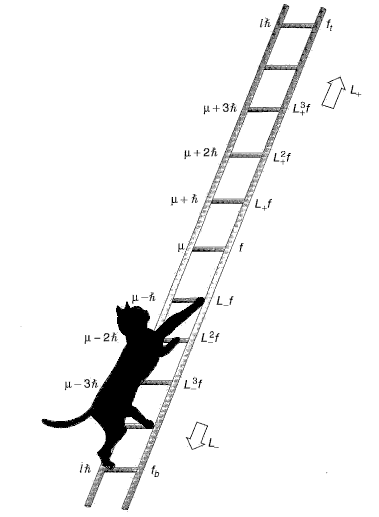
\includegraphics[scale=0.6]{Imagenes/Operadores_Escalera_01.png}
    \caption{La \enquote{escalera} de los estados del momento angular.}
    \label{fig:figura_escalera_01}
\end{figure}
Para un valor dado de $\lambda$, Entonces, obtenemos una \enquote{escalera} de estados, con cada \enquote{peldaño} separado de sus vecinos por una unidad de $h$ en el valor propio de $L_{z}$ (fig. \ref{fig:figura_escalera_01}). Para subir la escalera aplicamos el operador de ascenso, y para descender, el operador de descenso. Pero este proceso no puede continuar para siempre: eventualmente vamos a alcanzar un estado en el que el componente $z$ exceda el \emph{total}, y eso no puede ser. Debe existir un \enquote{escalón tope}, $f_{t}$, tal que:
\begin{align}
L_{+} \, f_{t} = 0
\label{eq:ecuacion_04_110}
\end{align}
Dejemos que $\hbar \, \ell$ sea un valor propio de $L_{z}$ en ese escalón tope (lo apropiado de la letra \enquote{$\ell$} se verá en un momento):
\begin{align}
L_{z} \, f_{t} = \hbar \, \ell \, f_{t}, \hspace{1.5cm} \vb{L}^{2} \, f_{t} = \lambda \, f_{t}
\label{eq:ecuacion_04_111}
\end{align}
Ahora:
\begin{align*}
L_{\pm} \, L_{\mp} &= (L_{x} \pm i \, L_{y})(L_{x} \mp i \, L_{y}) = \\[0.5em] 
&= L_{x}^{2} + L_{y}^{2} \mp i (L_{x} \, L_{y} - L_{y} \, L_{x}) = \\[0.5em]
&= \vb{L}^{2} - L_{z}^{2} i (\mp i \, \hbar \, L_{z})
\end{align*}
o dejándolo de otra manera:
\begin{align}
\vb{L}^{2} = L_{\pm} \, L_{\mp} + L_{z}^{2} \mp \hbar \, L_{z}
\label{eq:ecuacion_04_112}
\end{align}
Se sigue entonces que:
\begin{align*}
\vb{L} \, f_{t} &= (L_{-} \, L_{+} + L_{z}^{2} + \hbar \, L_{z}) \, f_{t} = \\[0.5em]
&= (0 + \hbar^{2} \, \ell^{2} + \hbar^{2} \, \ell) \, f_{t} = \\[0.5em]
&= \hbar^{2} \, \ell (\ell + 1) \, f_{t}
\end{align*}
de aquí
\begin{align}
\lambda = \hbar^{2} \, \ell (\ell + 1)
\label{eq:ecuacion_04_113}
\end{align}
Esto nos da el valor propio de $\vb{L}^{2}$ en términos del máximo valor propio de $L_{z}$.
\par
Mientras tanto, también hay (por la misma razón) un \emph{escalón inferior}: $f_{b}$, tal que
\begin{align}
L_{-} \, f_{b} = 0
\label{eq:ecuacion_04_114}
\end{align}
Sea $\hbar \, \overline{\ell}$ el valor propio de $L_{z}$ en este escalón inferior:
\begin{align}
L_{z} \, f_{b} = \hbar \, \overline{\ell} \, f_{b}, \hspace{1.5cm} \vb{L}^{2} \, f_{b} = \lambda \, f_{b}
\label{eq:ecuacion_04_115}
\end{align}
Usando la ec. (\ref{eq:ecuacion_04_112}), tenemos que:
\begin{align*}
\vb{L} \, f_{b} &= (L_{+} \, L_{-} + L_{z}^{2} - \hbar \, L_{z}) \, f_{b} = \\[0.5em]
&= (0 + \hbar^{2} \, \overline{\ell}^{2} - \hbar^{2} \, \overline{\ell}) \, f_{b} = \\[0.5em]
&= \hbar^{2} \, \overline{\ell} (\overline{\ell} - 1) \, f_{b}
\end{align*}
por lo tanto:
\begin{align}
\lambda = \hbar^{2} \, \overline{\ell} (\overline{\ell} - 1)
\label{eq:ecuacion_04_116}
\end{align}
Al comparar las ecuaciones (\ref{eq:ecuacion_04_113}) y (\ref{eq:ecuacion_04_116}), vemos que
\begin{align*}
\ell (\ell + 1) = \overline{\ell} (\overline{\ell} + 1)
\end{align*}
por lo que $\overline{\ell} = \ell + 1$, lo cual es absurdo: ¡el escalón inferior sería más alto que el escalón superior!, o que:
\begin{align}
\overline{\ell} = - \ell
\label{eq:ecuacion_04_117}
\end{align}
Evidentemente, los valores propios de $L_{z}$ son $m \, \hbar$, donde $m$ (la idoneidad de esta letra también será clara en un momento) va de $-\ell$ a $+\ell$ en $N$ pasos enteros. En particular, se deduce que $\ell = -\ell + N$, y por tanto $\ell = N/2$, por lo que $\ell$ debe ser un \emph{número entero o semi entero}. Las funciones propias se caracterizan por los números $\ell$ y $m$:
\begin{align}
\setlength{\fboxsep}{3\fboxsep}\boxed{
\vb{L}^{2} \, f_{\ell}^{m} = \hbar^{2} \, \ell (\ell + 1) \, f_{\ell}^{m} \hspace{1cm} \vb{L}_{z} \, f_{\ell}^{m} = \hbar \, m \, f_{\ell}^{m}
}
\label{eq:ecuacion_04_118}
\end{align}
donde
\begin{align}
\begin{aligned}
\ell &= 0, \dfrac{1}{2}, 1, \dfrac{3}{2}, \ldots \\[0.5em]
m &= -\ell, -\ell + 1, \ldots, \ell -1, \ell
\end{aligned}
\label{eq:ecuacion_04_199}
\end{align}
Para un valor dado de $\ell$, hay $2 \, \ell + 1$ valores diferentes de $m$ (es decir, $2 \, \ell + 1$ \enquote{escalones} en la \enquote{escalera}).
\par
A algunas personas les gusta ilustrar este resultado con el diagrama de la figura (xx) (dibujado para el caso $\ell = 2$). Se supone que las flechas representan los posibles momentos angulares en unidades de $\hbar$, todas tienen la misma longitud $\sqrt{\ell (\ell + 1)}$ (en este caso $\sqrt{6}= 2.45$), y sus componentes $z$ son los valores permitidos de $m  (-2, -1, 0, 1, 2)$. 
\begin{figure}[H]
    \centering
    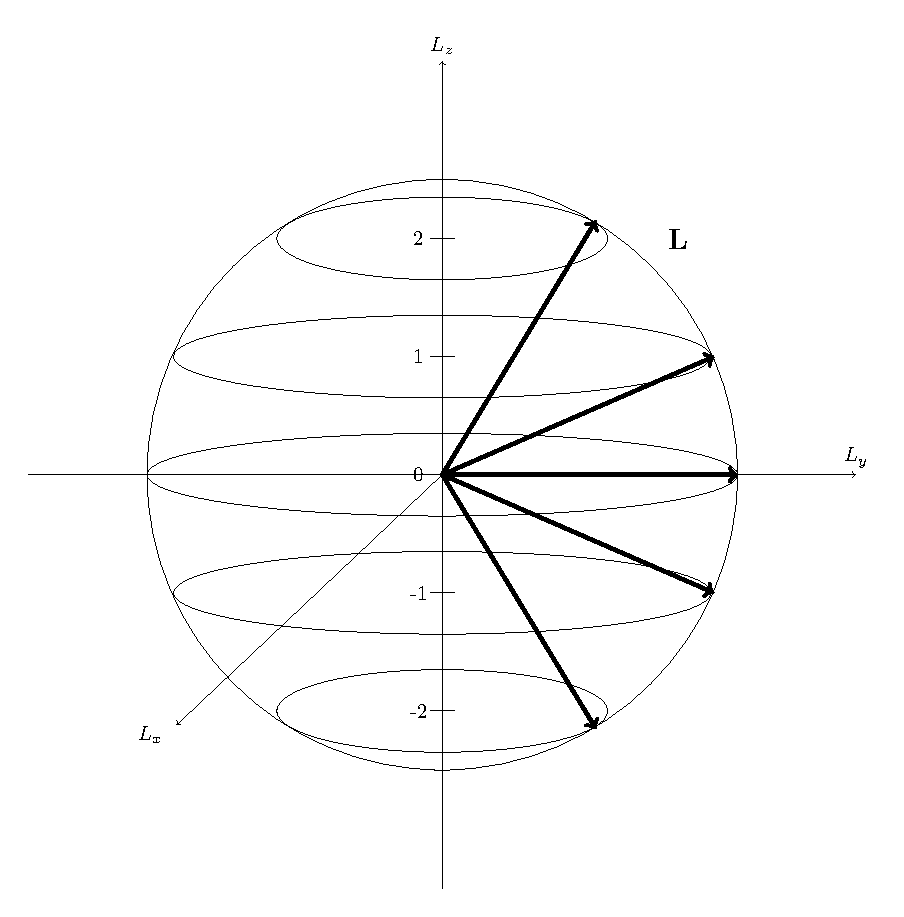
\includegraphics[scale=0.75]{Imagenes/Momento_angular_01.eps}
    \caption{Estados para el momento angular (con $\ell=2$).}
    \label{fig:momento_angular_02}
\end{figure}

Notése que la magnitud de los vectores (el radio de la esfera) es mayor que la componente $z$ máxima. (En general, $\sqrt{\ell (\ell + 1)} > 1$, excepto en el caso \enquote{trivial} $\ell = 0$.) Evidentemente, no se puede hacer que el momento angular apunte perfectamente a lo largo de la dirección $z$. Al principio, esto suena absurdo. \enquote{¿Por qué no puedo simplemente elegir mis ejes de modo que $z$ apunte a lo largo de la dirección del vector de momento angular?}. Bueno, para hacer esto tendríamos que conocer las tres componentes simultáneamente, y el principio de incertidumbre 
\begin{align}
\sigma_{L_{x}} \, \sigma_{L_{y}} \geq \dfrac{\hbar}{2} \, \abs{ \expval{L_{z}}}
\label{eq:ecuacion_04_100}
\end{align}
dice que eso es imposible. \enquote{Bueno, está bien, pero seguramente de vez en cuando, por suerte, apuntaré mi eje $z$ en la dirección de $\vb{L}$}. No, no! te has perdido el punto.
\par
No es simplemente que no conozcas las tres componentes de $\vb{L}$; simplemente no hay tres componentes: una partícula no puede \emph{tener} un vector de momento angular determinado, como tampoco puede tener simultáneamente una posición y un momento determinados. Si $L_{z}$ tiene un valor bien definido, entonces $L_{x}$ y $L_{y}$ no lo tienen. Es engañoso incluso dibujar los vectores en la figura xx; en el mejor de los casos, deberían estar distribuidos alrededor de las líneas de latitud, para indicar que $L_{x}$ y $L_{y}$ son indeterminados.
\par
Por medios puramente algebraicos, comenzando con las relaciones de conmutación fundamentales para el momento angular, se han determinado los valores propios de $\vb{L}^{2}$ y $L_{z}$, ¡sin siquiera ver las funciones propias!
\par
Pasamos ahora al problema de construir las funciones propias, pero hay que tomar en cuenta que este es un asunto mucho más complicado. Veamos hacia dónde nos dirigimos: $f_{l}^{m} = Y_{\ell}^{m}$: las funciones propias de $\vb{L}^{2}$ y $L_{z}$ no son más que los \emph{armónicos esféricos}, éstos son ortogonales: son funciones propias de operadores hermitianos ($\vb{L}^{2}$ y $L_{z}$) que pertenecen a valores propios distintos.

\end{document}